\subsection{Избор на IDE}
За да можем да създаваме софтуер на Rust, по най-ефективния начин се нуждаем от
текстов редактор който поддържа LSP. LSP или Language Server Protocol е
протокол създаден от Microsoft за Visual Studio Code и служи за комуникация
между техтовят редактор и специализирани програми, които анализират кода който
пишем и показват къде има грешки, предложения как да бъдат поправени, допълване
на код, подчертаване на синтаксиса \cite{lsp_wikipedia}.

\subsubsection{Visual Studio Code}
Visual Studio Code е текстов редактор с отворен код създаден от Microsoft. Той
използва Electron за графична библиотека и работи на Windows, Linux и MacOS. 
През 2022 в допитване до потребителите на Stack Overflow, Visual Studio Code е
класиран като най-популярният текстов редакор сред 71 010 респонденти
\cite{vscode_wikipedia}.

Visual Studio Code със заводските си настройки неможе да прави почти нищо. За
да получим всички полезни функционалности на LSP, трябва да инсталираме така
наречените плъгини.
% TODO: add images; how to install rust-analyzer etc.

Един от недостатъцине на VSCode обаче е високите системни изисквания за
нормална работа и моментално време за реакция при въвеждане на текст.
\begin{figure}[!htb]
  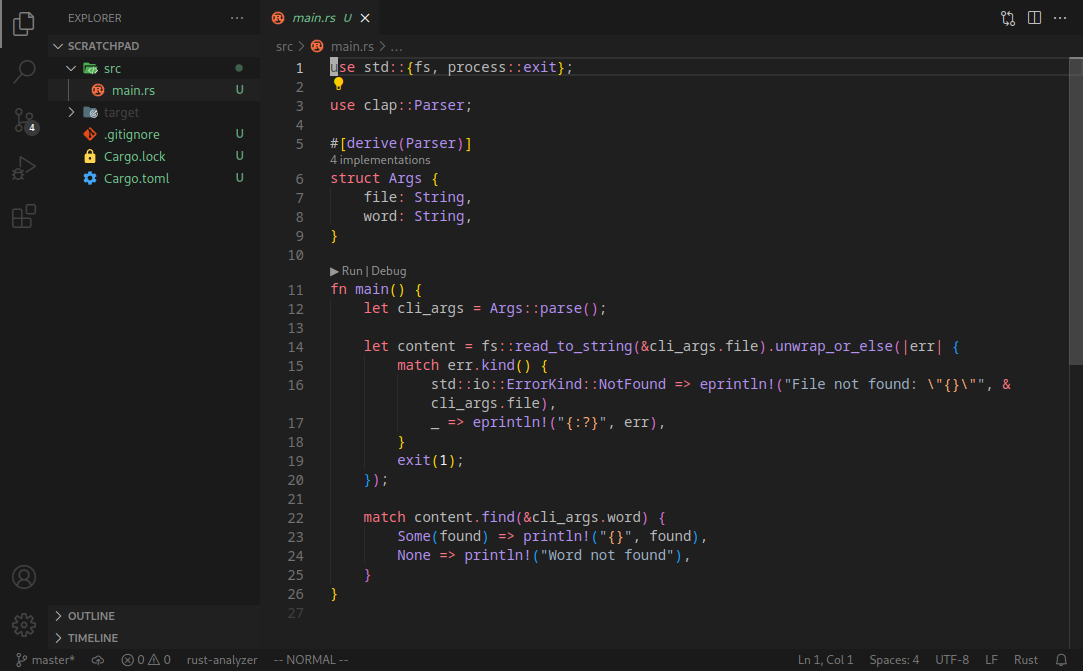
\includegraphics[scale=0.40]{vscode}
  \centering
  \caption{Visual Studio Code}
  \label{fig:vscode}
\end{figure}

\subsubsection{Vim}
Vim e техтов редактор с отворен код първоначално написан за настолният компютър
Amiga\cite{amiga_wikipedia} през 1991 година от Брам Моленар. За разлика от
Visual Studio Code, vim e текстов редактор, който e бил замислен да работи не
само в графичти среди, но и в терминални среди \cite{vim_wikipedia}. 

Най-привекателната част от Vim е начина за навигация. В повечето редктори се
навигира чрез мишката и няколко клавишни комбинации, докато Vim използва само
клавишни комбинации. По този начин ръцете ни остава на клавиатурата и няма
нужда да отделяме време за навигиране с мишка. 

Vim разполага с 3 режима за работа и това са:
\begin{itemize}
\item Normal - В нормалният режим можем само да манипулираме текст
\item Visual - В визуалният режим можем да избираме по-голими региони от текст
\item Command - В командният режим можем да изпълняваме команди за манипулиране
на текст, настройване на редактора и изпълнение на команди в операционната
система \end{itemize}

Vim успява да много малко ресурси от VSCode, без да прави компромиси от към
функционалности. За да може да бъде постигнато Vim е написан на C и потребителя
трябва ръчно да си настрои редактора, използвайки специално направеният език
VimScript. Този процес е прекалено сложен за повечето потребители затова те
предпочитат да използват VSCode, дори и да използва повече ресурси.

\subsubsection{Neovim}
Neovim е копие на Vim, което се стреми да подобри скороста и поддръжката на
Vim. Някои добавени функционалности на копието включват вградена поддръжка на
LSP и поддръжка за Lua скриптове като заместител на VimScript \cite{neovim_wikipedia}.

Проектът Neovim стартира през 2014 година, като някои членове на Vim общността
предлагат помощ в усилията за основно рефакториране, за да осигурят по-добри
eзици за скриптове, плъгини и интеграция с модерни графични потребителски интерфейси.
Проектът е с отворен код и, който е достъпен в GitHub. \cite{neovim_github}

От към производителност Neovim е малко по-бавен от предшественика си Vim, но
все пак е в пъти по-бърз от главния си конкурен Visual Studio Code, затова аз
се спрях на Neovim.

\begin{figure}[!htb]
  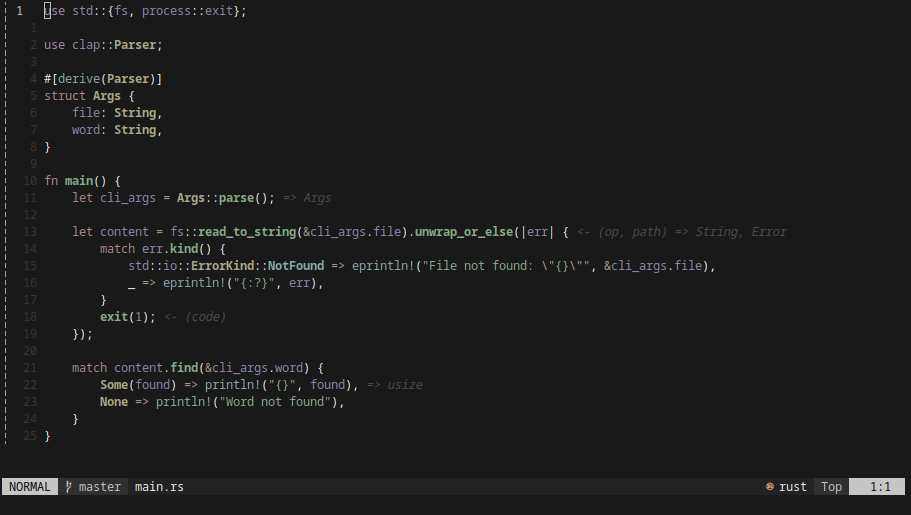
\includegraphics[scale=0.50]{neovim}
  \centering
  \caption{Neovim}
  \label{fig:neovim}
\end{figure}

\subsection{Git}
Git е система за контрол на версиите, която проследява промените във всеки
набор от компютърни файлове, обикновено се използва за координиране на работата
между програмистите, които съвместно разработват изходния код по време на
разработката на софтуер. Целите на системата включват скорост, цялост на
данните и поддръжка за разпределени, нелинейни работни потоци (хиляди паралелни
клонове, работещи на различни системи).

Git първоначално е създаден от Линус Торвалдс, през 2005 година за разработване
на ядрото на Linux, като инструмен за други разработчици на ядрото да
допринасят за първоначалното му развитие. От 2005 година Junio Hamano е основният
разработчик. Както при повечето други разпределени системи за контрол на версиите
и за разлика от повечето системи клиент-сървър, всяка Git директория на всеки
компютър е пълноценно хранилище с пълна история и пълни възможности за
проследяване на версиите, независимо от достъпа до мрежата или централен
сървър. Git е безплатен софтуер с отворен код, разпространяван само под лиценз
GPL-2.0. \cite{git_wikipedia}
